 \documentclass[conference]{IEEEtran}

\ifCLASSINFOpdf
\usepackage[pdftex]{graphicx, hyperref}
\DeclareGraphicsExtensions{.pdf,.png,.jpg}
\usepackage{listings}
\fi

\usepackage{zed} % version 4 included in directory

\newtheorem{definition}{Definition}

\begin{document} 

\title{Model Driven Engineering for \\ Large-Scale Clinical Research}

\vskip 4mm 

\author{%
  \IEEEauthorblockN{Jim Davies, Jeremy Gibbons, David Milward,
    Seyyed Shah, Monika Solanki, and James Welch%
  }
  % 
  \IEEEauthorblockA{%
    Department of Computer Science, University of Oxford \\
    Email: \texttt{Firstname.Lastname@cs.ox.ac.uk}
  }
}

\ifpdf
\graphicspath{{ASEFigs/}}
\fi

\maketitle

\begin{abstract}
  Scientific progress in medicine is increasingly dependent upon the
  large-scale integration of data from a range of sources.  This data
  is acquired in different contexts, held in different systems, and
  subject to different processes and constraints.  The value of the
  integrated data relies upon common data points having a consistent
  interpretation in each case; to achieve this at scale requires
  appropriate informatics support.  This paper explains how a
  model-driven approach to software engineering and data management,
  in which software artefacts are generated automatically from data
  models, can be used to achieve this.  It introduces a simple data
  modelling language, consistent with standard object modelling
  notations, together with a set of tools for model creation,
  maintenance, and deployment.  It reports upon the application of
  this approach in the provision of informatics support for two
  large-scale clinical research initiatives.
\end{abstract}

\vskip 14mm

\noindent

\section{Introduction}

Scientific progress in medicine consists principally in the
introduction of new diagnostics and new therapeutics: new ways of
figuring out what is wrong, and new ways of doing something about it.
The causes of disease, the expression of symptoms, and the response to
treatment, can be extremely complex, involving many levels of
biology---genomics, proteomics, metabolomics---and a wide variety of
lifestyle and environmental factors.

To obtain the evidence to support the introduction of a new diagnostic
or therapeutic, while taking account of the variations in biology and
environment, we need to make detailed, comparable observations of a
suitably large number of individuals.  These observations will be made
by different people, under different circumstances, and stored and
processed in different information systems.  A significant degree of
coordination is required to achieve an adequate combination of detail
and comparability.

One means of achieving this involves prior agreement upon a prescribed
dataset: a precise specification of the observations needed to answer
a particular question.  An information system is then implemented or
configured to match this dataset, and staff are trained to acquire
data to match the prescribed interpretation.  This can be
time-consuming and expensive.  Furthermore, the data acquired is
unlikely to be re-used: not only is the dataset as a whole tailored
towards a particular question, but the same may be true of the
individual observations.

It should be clear that this is unnecessary.  A dataset can be
composed by drawing upon, and adding to, a library of existing data
definitions.  As a precise specification, it can be used as the basis
for the automatic generation or configuration of an information system
for data capture, reducing costs while enhancing the value of the data
obtained.  The enhanced value comes in part from the fact that some of
the data has been recorded against existing definitions, but also from
the fact that definitions are readily available---in a re-usable,
computable form---for all of the data collected.

Costs can be further reduced, and scientific progress accelerated, by
re-using data already collected: in other scientific studies; in the
course of care delivery; or from other sources, including new sensor
technologies.  Precise data definitions are important here also: we
need to know whether the data already collected is fit for purpose,
whether its interpretation is consistent with the analysis that we
intend to perform.  In most cases, these definitions will be created
retrospectively, by progressively adding information about the context
of collection, and any subsequent processing, until the interpretation
of the data is clear.

Having created precise definitions for existing data, we can enhance
the value of the data, and reduce the costs of research, by making
these definitions available in a standardised, computable form.  In
designing and proposing a new clinical study, researchers can take
account not only of what questions have been asked before, but also of
what data already exists, in other research databases or in clinical
information systems.  In this way, we can eliminate unhelpful
variation in study design and unnecessary duplication of effort in
data collection.

Furthermore, if we have both precise definitions of existing data, and
precise definitions of data requirements for a study, then we can
provide automatic support for aspects of study design and delivery:
definitions can be compared, queries can be generated for data
extraction, and---if summary metadata on the contents of existing
databases is available---the feasibility of a particular study can be
assessed in advance.

Scientific progress in medicine is increasingly dependent upon this
kind of automatic support for data management and integration.
Without it, we will be unable to assemble the evidence
needed---detailed, comparable data on thousands or millions of
individuals---to produce new insights, to validate new discoveries,
and to support the introduction of new diagnostics and therapeutics
into clinical practice.


This paper explains how a model-driven approach to software and data
engineering can provide the support required for large-scale clinical
research.  It introduces a simple data modelling language, consistent
with standard object modelling notations, together with a set of tools
for model creation, maintenance, and deployment.  It then reports upon
the experience of applying these tools within two large-scale clinical
research initiatives.

One of these initiatives involves the re-use of data captured in
existing clinical information systems.  In the area of translational
research, in which new innovations are developed and evaluated in the
context of clinical practice (`from bench to bedside'), the data
needed to support the science is often the same as that needed to
support high-quality care delivery and service improvement.  In
existing clinical systems, however, the same observation may be
recorded in many different ways, and there are significant
challenges. 

The other involves the development of new information systems for data
acquisition and management, as well as the customisation and re-use of
existing systems wherever possible.  Here, the emphasis is upon
defining new, generic datasets, in specific therapeutic areas, with
the aim of supporting a wide range of studies using the data
collected.  A particular challenge for informatics development and
data re-use stems from the constant updating of these datasets to take
account of new knowledge, new constraints, and new objectives.

Together, these initiatives provide an initial validation of the
approach.  The software tools are in use by clinical researchers,
rather than the software engineers responsible for their design.  Data
is being collected to the definitions that they have produced, using
software that they have generated.  It is too early to undertake any
quantitative, comparative evaluation; however, it is our hope that a
report of the approach taken, and the experience gained thus far, will
be useful to those working in the field of automated software
engineering.

\section{The Models Catalogue Language and Architecture}
 
\subsection{Models Catalogue}
A software \emph{model} is an abstraction of a software program, which will be instantiated and run using \emph{real data}, software modelling is becoming important for a number of reasons, not least that it enables developers the opportunity to \emph{re-use} code. The Unified Modelling Language UML \cite{UML} or Ecore \cite{ECORE} ( a subset of UML) are in widespread use for defining and representing software \emph{models}. UML and Ecore are defined at a level which is \emph{more abstract} than the model itself, and one which we term the \emph{meta-modelling} layer. 

The data we have been dealing with in these projects is mostly in the form of textual forms, sometimes in word or PDF format, sometimes in a more specialised form of XML or Excel. The data therefore does have a clear structure, although the clinician running the trial very often has little visibility, knowledge or appreciation of how the data is stored, and who else might in future want to access or manipulate that data.  Although the healthcare providers have work-flows which the patients and doctors follow in the treatment cycle, these are not being considered in this paper.

Sometimes there are standards available governing aspects of the data in question, for instance reporting of a particular clinical trial may need to be in XML which conforms to a particular XSD, however that doesn't mean that the data has been collected with that particular standard in mind.  For the most part clinicians are interested in fairly static data sets, a patient record, the results of a treatment, a clinical trial form, the dynamic aspects are less important, at any rate in terms of the computational representation. What is important is the meaning of the data once it is captured, and in particular how it relates to other data in the same field, for instance is \emph{tumour weight} in one experiment the same as \emph{tumour weight} in another. These two terms may be used in different contexts, for instance prostate cancer and liver cancer, and they may be represented by different values domain in different hospital trusts, for instance one may use grams the other kilograms, the values may be comparable but an adjustment will need to be made to make that comparison.

Thus there are two things we need to identify and reference in building the toolkit, firstly does this \emph{concept} \textbf{mean} the same as that \emph{concept}, and secondly does this \emph{concept} have the same \emph{representation} as that concept. The way in which we can match up concepts in software engineering is by associated them with classes of software objects, and then defining methods which can reference them. 

\subsection{ISO11179}
ISO11179 is the international standard relating to metadata and in particular metadata registries. It forms the basis of the design of the models catalogue toolkit.

\begin{figure}[here]
	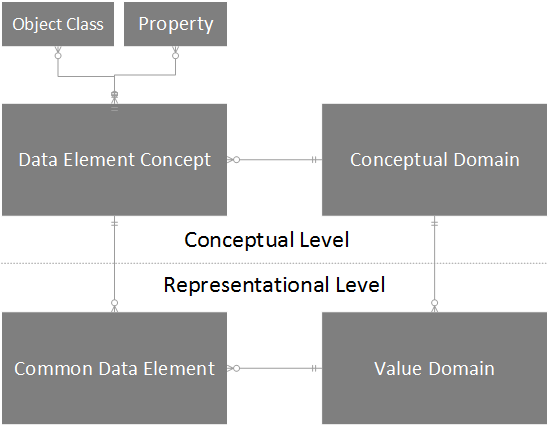
\includegraphics[width=0.48\textwidth,natwidth=610,natheight=642]{BasicISO}
	\caption{Core model for ISO11179 Metadata Registry} 
	\label{fig:basicMDR}
\end{figure}

The ISO11179 standard uses the notion of a \emph{data element concept}, \emph{a data element}, \emph{a value domain}, and a \emph{conceptual domain}. The standard currently confines itself to the detailed level of concepts and data elements and has no notion of collections of data elements or data element concepts, but instead attaches two attributes: an \emph{object class} and a \emph{property} to each data element concept and these attributes allow the data element concept's to be aggregated or classified. This core model of the ISO11179 is illustrated in figure \ref{fig:basicMDR}. The data element concept and conceptual domain entities belong to the \emph{conceptual level}  whilst the common data element and value domain both belong to the \emph{representational level}.


For example an Integer data-type in a programming language may be used to represent inches in a measurement program, it may also be used to count vehicles in a logistics application.  A data element is said to be comprised of a data element concept(DEC) which is its meaning and a value domain(VD) which is its representation.

\begin{table}[h]
	\begin{tabular}{ p{1.8cm} p{2.8cm}  p{3.0cm}  }  % centered columns (2 columns)
		\hline
		Entity & ISO Definition & ISO11179 Implementation Guidelines  \\ 
		\hline
		Data Element Concept(DEC) & An idea that can be represented in the form of a data element, described independently of any particular representation. & A concept that can be represented in the form of a Data Element, described independently of any particular representation.\\
		Common Data Element(CDE) & A unit of data for which the definition, identification, representation, and permissible values are specified by means of a set of attributes. & A unit of data for which the definition, identification, representation and Permissible Values are specified by means of a set of attributes. \\
		Value Domain (VD) & The description of a value meaning. & A description of a Value Meaning. \\
		Conceptual Domain (CD) & A set of valid value meanings, which may be enumerated or expressed via a description.& A set of valid Value Meanings.\\
		\hline
	\end{tabular}
\end{table}

The table lists the definitions of the key entities used in the standard
Conceptual domains comprise sets of value domains, they provide a collection mechanism of \emph{Value Meanings} which provide representation for a particular data element concepts. Data Element Concepts can then be grouped according to their Object Class, or Property, however whilst this works for a system that is focussed entirely on the metadata units, any working software system will need to group the data elements in a structure that is easily transformed into the components such as Classes and Entities that are used in most information systems.   



\subsection{A Metadata Language and Abstract Architecture }

The ISO11179 specification illustrates different aspects of the standard using UML class diagrams, and we have used these to inform the development of a very simple domain specific language for metadata, which we are calling the \emph{Language for Enterprise Metadata Modelling LEMM}. The next section gives a description of the language and highlights how it differs from the meta-model outlined in the standard. Probably the key changes are that we have added in containers to handle data element collections, calling these \emph{DataClasses} and to handle collections of these \emph{DataClasses} which we have introduced entities called \emph{DataModels}.

A simplified overview model, without attributes and methods, showing the Ecore model for the LEMM DSL is shown in Figure \ref{fig:mcSimplifiedOverview}.

\begin{figure}[here]
	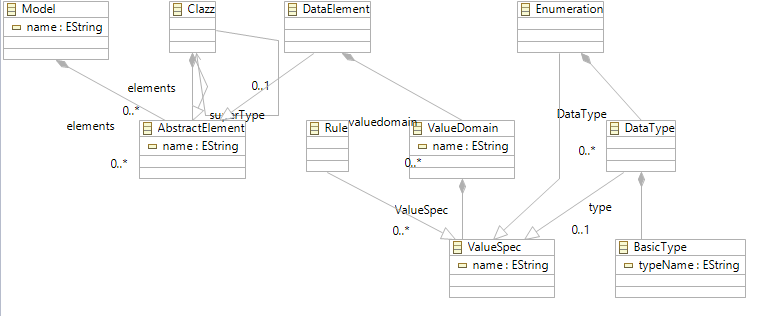
\includegraphics[width=0.5\textwidth,natwidth=610,natheight=642]{ELM_EcoreDiagram}
	\caption{Overview of LEMM in Ecore} 
	\label{fig:mcSimplifiedOverview}
\end{figure}

\subsubsection{DataModel}
A datamodel is a grouping or containment entity which groups a set of \emph{DataClasses} together. DataModels can be thought of as datasets, or even database schemas, very often in the medical domain they are defined either by XML Schema definition files, or by equivalent schemas written in Excel. 
DataModels are collections of \emph{ConceptElements} which in turn can be either \emph{Data Elements} or \emph{Classes}. There is no real notion of composition or multiplicity, a instance of a DataModel can contain an instance of a Data Element or not as required by the instance.  DataModels are named, have a description and have a version identity.
\subsubsection{DataClass}
A DataClass is a grouping or collection of \emph{attributes} which can be data elements or classes, the attributes are currently \emph{mandatory}, so that DataClass with 5 attributes must have those 5 attributes instantiated in an instance for it to be considered of that DataClass. A dataclass is named to differentiate it from the term \emph{Class} as used in object oriented programming languages, it captures the structural rather than behavioural aspects of a class.  DataClasses represent \emph{Concepts}, and can be \emph{Generalized} into a hierarchy, giving some of the benefits of inheritance to the language.  
\subsection{Data Elements} 
Data Elements can also represent \emph{Concepts} and are by their nature \emph{atomic}.  Each data element is related to a value domain on a one-to-one basis, and the relationship is a two-way relationship.
\subsection{Value Domain}
A Value Domain is the domain in which the data element is represented, it can consist of one or more \emph{ValueSpecs}.
\subsection{ValueSpec}
A \emph{ValueSpec} can be a simple datatype, an enumeration of datatypes, or a rule - such as a regular expression - which defines the way in which a series of characters is formed into a string attribute. 


\lstinputlisting[label=elm,caption=Language for Enterprise Modelling]{ASEFigs/ElmmDSL.xtext}

<<<<<<< Updated upstream
The ElmDSL is used to represent a model for Cancer data (part of the Cancer Outcomes and Services Dataset \cite(COSD)) in Figure \ref{fig:elmcosd}

\begin{figure}[here]
	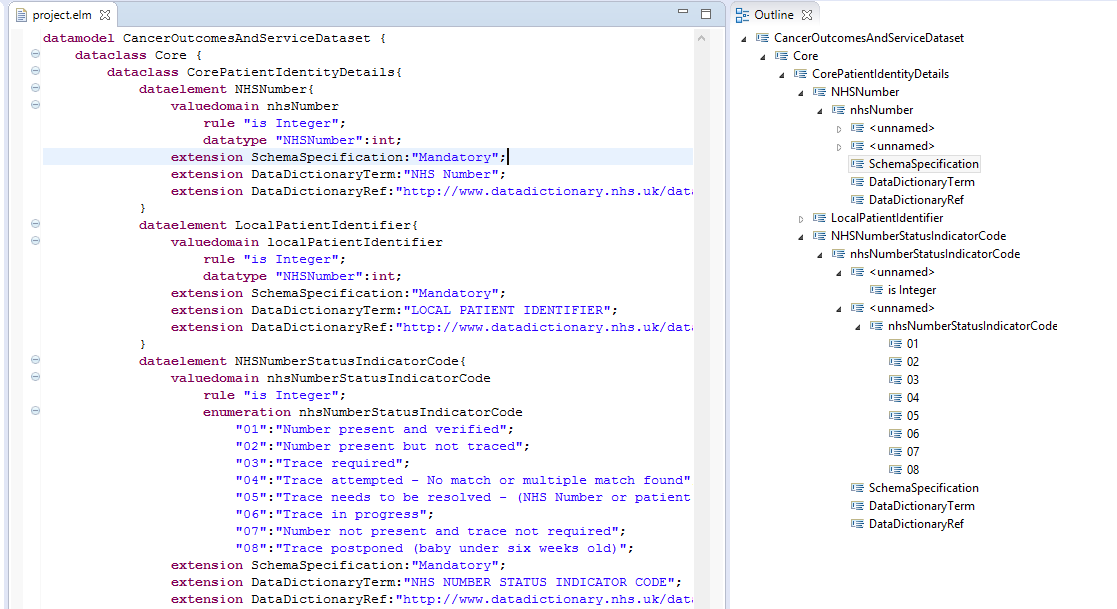
\includegraphics[width=0.5\textwidth,natwidth=610,natheight=642]{ElmDSLCOSDModel}
	\caption{COSD data in LEMM Model} 
	\label{fig:elmcosd}
\end{figure}

The original dataset was collected and managed in Excel, as shown in Figure \ref{fig:excelCOSD}

\begin{figure}[here]
	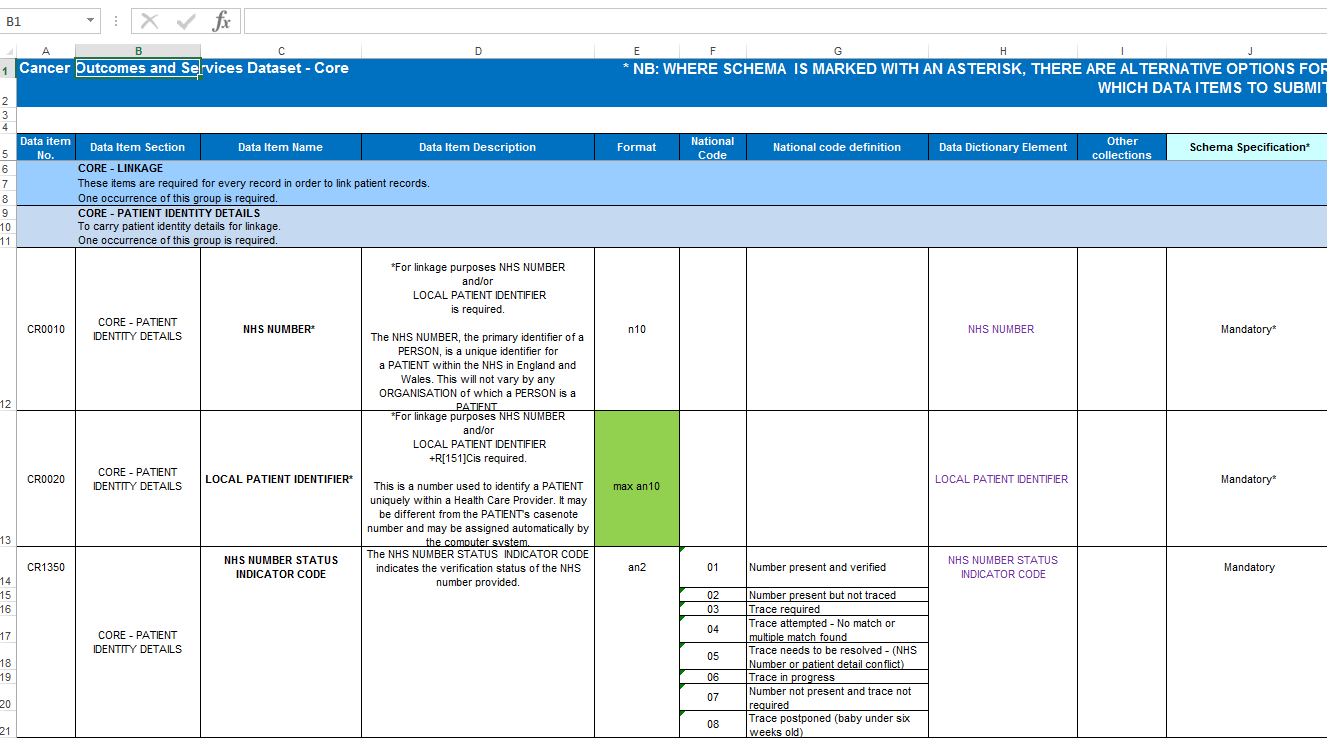
\includegraphics[width=0.5\textwidth,natwidth=610,natheight=642]{COSDExcel}
	\caption{COSD data in Excel Format} 
	\label{fig:excelCOSD}
\end{figure}


=======
>>>>>>> Stashed changes

\section{Implementation}

Groovy was chosen as a language for implementation for two reasons, firstly
it has a very efficient web framework called Grails built on the Spring framework,
which is not only proven to be very robust and scalable, but is also
very easy to implement and so enables quick development cycles. Previous
implementations using Java/Spring and Java/Roo have proved very timeconsuming
to experiment with, Grails has proven to be very flexible. The
second reason was that Grails offers both functional capability, and dynamic
meta-programming capability. This means that DSL’s can be easily built on
this framework, something that hasn’t been used yet, but will be needed when
the automatic forms generation capability is added. At this stage I have built 2
forms generating DSLs, although must more work will be required to get one
that can implement automatic forms generation.
 
The MDR implementation discussed here has been implemented using the
Groovy programming language, and the Grails Framework and is based on
the concepts put forward in the ISO11179 standard. There are a few changes
to basic model in that the idea of a Data Element Concept has been merged
with the idea of aModel. Data Elements have been retained, and they are related
to both aModel and a Value Domain. Models can contain other models,
and are essentially the basic building block of the data definitions, however
at their lowest resolution a model will be composed of a Data Element and at
least one Value Domain.
 
\section{Experience}

Key ideas:

\begin{itemize}
	\item Data Elements can be used across different DataModels - favourites or shopping cart.
	\item Unique Identification of DataElements 
	\item Documentation can be automatically generated for review purposes
	\item Consistency checking carried out on data elements
	\item Generation of XSDs, XML, and Forms as output, interfacing with OpenClinica.
	\item Data Provenance
\end{itemize}


\subsection{NHIC}

The NIHR-funded HIC project is concerned with the creation of research
datasets in five key clinical domains: Acute Coronary Syndromes,
Hepatology, Intensive Care, Ovarian Cancer, and Renal Transplantation.
Each is to populated with data taken from routine clinical care, and
integrated across five of the largest teaching hospitals in the United
Kingdom.

This project provided a number of challenges:

\begin{itemize}
\item To define an appropriate dataset for each of the five themes
  that could be re-used in future research studies, and linked to
  external data sources.
\item To understand and clarify the differences in data collection
  across the five sites, and record this in a suitable manner for
  researchers to review at a later date.
\item To define common data collection tools, such that each site
  could collate and submit their own data to the lead site.

\end{itemize}

In each theme, the process of data-modelling started with the
identification of key data points that are recognised as important for
all research in that domain.  For example in Cancer treatment, the
size and shape of any tumour before and after any intervention are
important.  This process was primarily carried out by domain-experts -
the academic clinicians with a knowledge of the data required for
research, and the data collected during core clinical care.  Also
involved in the process were nurses responsible for collecting the
data in routine care of clinical trials, the researchers involved in
disseminating data in trials, and the IT staff charged with storing
and collating data, who understand what may be available.

Most of this initial modeling was carried out via Excel spreadsheets:
many existing datasets are defined in this form and so was familiar to
the domain experts.  We built an importer for the model catalogue that
allowed these Excel spreadsheets to be parsed and stored according to
the Model Catalogue schema.  We recorded links between datapoints in
the HIC datasets and those in pre-existing reporting datasets.  In
some cases these were auto-detected, in some cases recorded manually
through the model catalogue interface, and in some cases these were
imported via the Excel documents.  

In each theme, existing datasets had already been defined, with the
purpose of providing summary data for hospitals charging services, or
for national reporting against predefined targets.  In many cases
these data points were a good starting point for a research dataset,
but data collected was not sufficiently granular, or additional
data points were required for the purposes of clinical research.

For each data point, the sites recorded how that data was collected.
In the simplest case, that would include the value domain, and any
constraints on allowable values imposed by the collection tool.  It
became apparent that different sites may collect the same data point
according to different enumerated domains.  Where these values were
later submitted as part of, for example, a national reporting dataset,
these values would be translated, often resulting in a loss of
fidelity.  

It was clear that such transformations, and unification across a
number of different sites led to a great loss in information; each
data point being reduced to a lowest-common denominator.  One of the
key principles of the HIC programme was that each site should submit
data in the way in which it was collected, and document in the model
catalogue the way in which it was recorded.


In conjunction with this process, an exercise was undertaken at each
site to audit the quality, coverage, and consistency of the data at
each data point.  This helped to inform a pragmatic set of data which
might prove to be valuable in the short-term.

Each theme then refined the datasets into a number of structured
models.  In the first instance, UML class diagrams were created,
showing grouping and multiplicities of data.  For example,
measurements corresponding to the size and shape of a tumour may be
grouped according to the particular tumour that is of interest.  A
patient may have a number of tumours, and for each tumour, the size
and shape may be mandatory fields.

Where appropriate, patient pathway models were created to add
additional context.  Similar to a workflow diagram, the patient
pathway models described the common routes through the care system
that a patient may take.  Each data point was associated with one or
more points on the diagram, indicating where each data point is
collected, and where it may be used later on in making a decision
about the particular treatment a patient is to receive.

These models were typically created by the technical team in
collaboration with the domain experts.  In many cases, the patient
pathways were more complex than the clinicians had realised - and the
process of creating the models helped both parties understand the
complexity of the domain.  The models are preserved in the catalogue
for future re-use.

In most cases, these models served as a general purpose description
for each clinical theme.  However, differences in treatment at
different sites often led to distinctions being made: different models
were required for different sites.  For example, the decision whether
a particular cancer patient would be treated with surgery or
chemotherapy may be made differently at different sites, thus changing
the meaning of any data subsequently collected about that patient.

For each theme, we generated an XML schema, allowing each site to
submit their data according to a common structure.   


\subsection{Genomics England - reuse of HIC Models}

One of the prime tasks of Genomics England (GEL) is to integrate a patient's clinical records with that patients genome, and use this integrated data to inform new clinical research primarily in the domain of genetic medicine. In order to do this GEL is assembling core datamodels, initially to classify clinical research in the area of rare diseases and in the area of cancer.  In order to do this clinicians were asked to assemble datamodels in excel and XML format, and attempt to arrive at an agreed datamodel for the two areas.  Initially this was carried out by assembling the subject matter experts in a conference room and then going through each item in turn. The process was quite time consuming and difficult, mostly because the users were mostly eminent clinicians and extremely busy, so that getting all the contributors in the same room at the same time was itself quite a difficult task to achieve.

Whilst that process was being carried out, some of these datasets were added to the Model Catalogue, and the subject matter experts were given visibility of the datasets already stored in the Model Catalogue. At this point the Model Catalogue was already loaded with datasets derived from the NHS Data disctionary such as COSD and from the results of the NHIC work. Use of the toolkut resulted in the users being able to very quickly assemble a new dataset from an existing dataset; they were then able to go through each data element in turn and compare it to an existing data element in another datamodel, a process that is illustrated in figure \ref{fig:dataClassComparison}.

For the Genomics England exercise the Models Catalogue has been had an added social networking feature added, allowing messaging forums to be automatically generated around a \emph{datamodel} or \emph{dataclass} . This allows users to develop a new draft datamodel, and then 

From looking at the datasets we can see that in the first 2 major datamodels produced X\% of data elements and dataclasses were derived from existing sources, a fact entirely due to the use of the Model Catalogue in the data curation process. Time to assemble a new datamodel has been cut from months to weeks as a result of having a single shared source for the datamodel, and having the means to electronically comment on and discuss datamodel development in real time as it is happening.



 Figure \ref{fig:dataClassComparison}
 \begin{figure}[here]
 	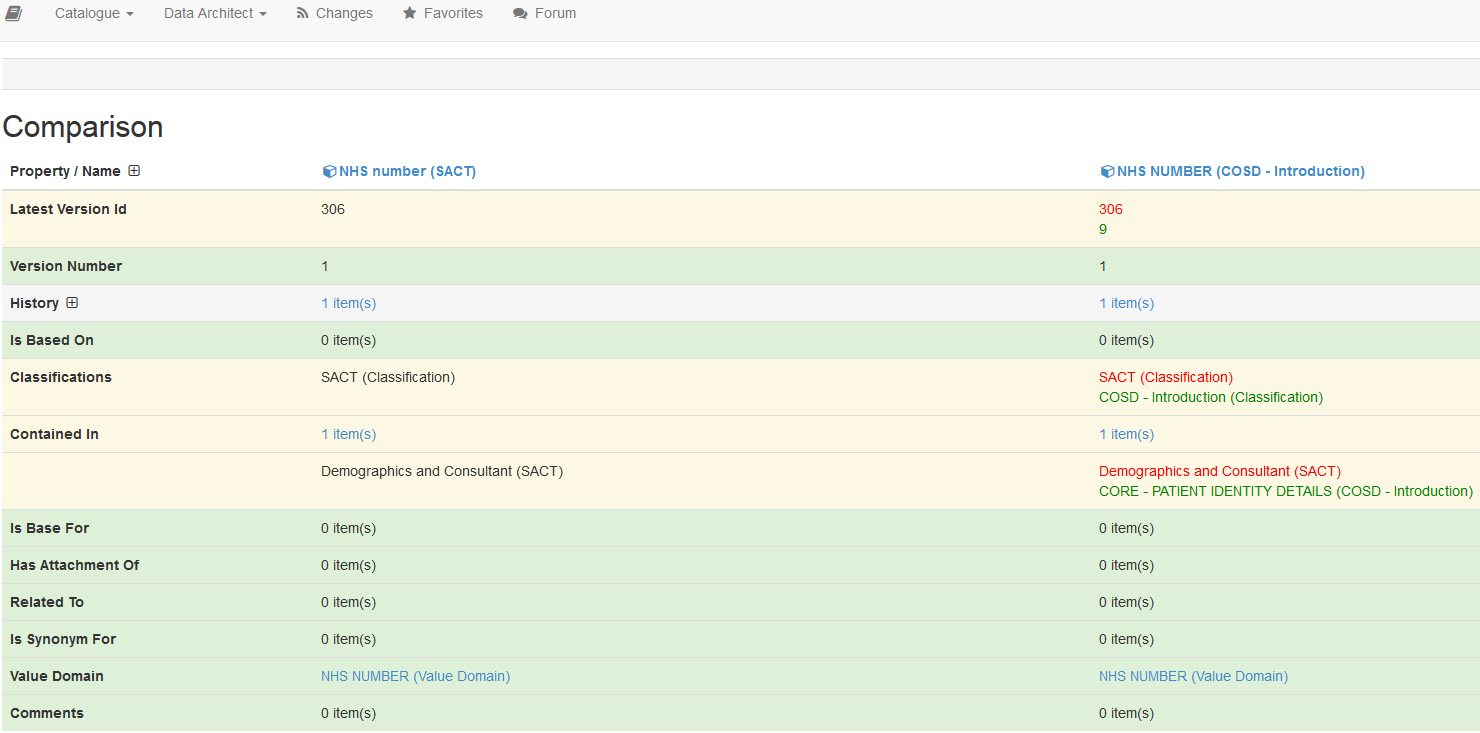
\includegraphics[width=0.5\textwidth,natwidth=610,natheight=642]{ComparisonOfDataClasses}
 	\caption{Screen Shot of DataClass Comparison} 
 	\label{fig:dataClassComparison}	
 \end{figure}



\subsection{Genomics England -  deployment}


\section{Related Work}

\subsection{ISO11179}

The work described in this paper has evolved from the CancerGrid
project~\cite{davi14}, where an ISO11179-compliant metadata registry
was developed for curation of semantic metadata and model-driven
generation of trial-specific software~\cite{davi12, Abler2011}. The
practical approach to generating forms in the CancerGrid project has
been made more formal in the current incarnation 
by use of an ISO11179-based metamodel, more
flexible by use of a plug-in architecture, and more scalable by use of a
collaborative on-line interface. 
%In techniques such as~\cite{mass13}, specific schemas recognised as a key
%component to enable large scale processing of genomic data, however
%the approach does not integrate ISO11179 principles and instead uses a
%single fixed schema for all data. 
Another effort to develop an
implementation of ISO11179 is found in the US caBIG
initiative~\cite{kunz09}; however, their 
caCORE software development kit~\cite{koma08}
applies model-driven development only to generate web service stubs,
requiring developers to create application logic by hand, whereas our
technique integrates with existing clinical Electronic Data Capture
tools and workflows, such as OpenClinica~\cite{oc}.

\subsection{Ontology modelling}

%%%% ontological representations of ISO11179 %%%%%%%%

Several efforts have addressed ontological representations of ISO11179 
for enabling data integration across metadata
registries (MDRs). Sinaci and Erturkmen~\cite{Sinaci2013784} describe a
federated semantic metadata registry framework where Common Data
Elements (CDEs) are exposed as Linked Open Data resources. CDEs are
described in the Resource Description Framework (RDF), and can be queried and interlinked with CDEs in other
registries using the W3C Simple Knowledge Organization System (SKOS). 
An ISO11179 ontology has been defined as part of
the framework, and the Semantic MDR has been implemented using the Jena
framework. 
Jeong \textit{et~al.}~\cite{pmid25405066} present the Clinical
Data Element Ontology (CDEO) for unified indexing and retrieval of
elements across MDRs; they organise and
represent CDEO concepts using SKOS. 
Tao \textit{et~al.}~\cite{pmid22211181} present
case studies in representing HL7 Detailed Clinical Models (DCMs) and
the ISO11179 model in the Web Ontology Language (OWL);
a combination of UML diagrams and Excel
spreadsheets were used to extract the metamodels for fourteen HL7 DCM
constructs. A critical limitation of this approach is that the
transformation from metamodels to their ontological representation in
OWL is based on a manual encoding. 
Leroux \textit{et~al.}~\cite{lero12} use existing
ontologies to enrich OpenClinica forms; our Model Catalogue
technique can integrate these ontologies to capture compliant data in
a similar fashion, but does so by using an ISO11179 meta data registry
and model driven methodology.

%%%% Ontology repositories %%%%%%%%%

Ontology repositories can be considered closely analogous to model
catalogues, they provide the infrastructure for storing, interlinking,
querying, versioning and visualising ontologies. Relationships
capturing the alignments and mappings between ontologies are also
captured, allowing easy navigability. Linked Open
Vocabularies~\cite{LOV} provides a service for discovering
vocabularies and ontologies published following the principles of
linked data. Besides the above features, it provides documentation
about ontologies automatically harvested from their structure and
identifies dependencies. Apache Stanbol~\cite{Stanbol} provides a set
of reusable components for semantic content management. The Apache
Stanbol Ontology Manager provides a controlled environment for
managing ontologies and ontology networks. 
%Main components of the
%manager include (a) Ontonet, a Java API for the construction and
%management of ontology networks from the ontology knowledge base. (b)
%Registry, an RDF resource that provides descriptions of ontology
%libraries in the knowledge base. The registry also provides a
%management API for administrators to pre-configure sets of ontologies
%loaded in the ontology libraries. KAON2~\cite{Kaon2} provides an API
%infrastructure for managing OWL-DL, SWRL and F-Logic
%ontologies. Access to the ontologies is provided via a single stand
%alone server. OWL DL Inferencing and SPARQL based querying are
%supported.


%%%%%%%%%%%%%%%%%%%%%%%%%%%%%%%%%

\subsection{Data warehousing}

In data warehousing~\cite{kim02}, metadata is modelled in order to copy
information from business systems into a centralised `data warehouse',
for decision support and to analyse business performance. Data
warehouse models can be arranged in normalised form, following the
relational approach~\cite{inm92}, or `dimensional' form~\cite{kim02}
as quantifiable \emph{facts} and \emph{dimensions} which denote the
context of facts. The Common Warehouse Metamodel (CWM)~\cite{poole03}
from the Object Management Group is a UML-based framework to enable
data warehousing in practice. Data warehousing is focused on
write-once models, and for working with rigidly structured data; this
is in contrast to the more general approach taken in ISO11179, where
models are expected to evolve and change over time. 
The core metamodel of the CWM standard overlaps with the 
\emph{concept} and \emph{value} elements of the ISO11179 meta model.

\subsection{Model-driven engineering for e-Health}

Several examples of model-driven engineering for e-Health software are
reported in the literature~\cite{dav14,ragh08,blob07,kham08,schl15}.
Payne~\cite{pay12} formalises the typical pattern followed in these
methods: a multi-phase approach, where data modelling is a separate
phase from stakeholder engagement and data integration. This approach
is taken Khambati \textit{et~al.}~\cite{kham08}, where an
Eclipse-based tool is used to develop domain-specific languages to
model and generate tools for mobile health-tracking applications. The
advantage of the approach is the ability it provides for clinicians to
modify the model of the study, which is specified in the DSL, and
automatically regenerate the application from the model. A similar
approach is taken in the \emph{True Colours} system~\cite{dav14},
using the Booster model-driven toolkit to derive a patient
self-monitoring application for mental health. The Booster approach
demonstrates the lesson that data tends to be managed better within a
model-driven process, leading to higher quality and more reusable
assets.  Schlieter \textit{et~al.}~\cite{schl15} record their
experience gained from using model-driven engineering to implement an
application for path-based stroke care; amongst the lessons learned,
they recommend using existing ontological models where possible, and
being prepared to reconcile a heterogeneity of models from the various
stakeholders under a common metamodel.  In contrast to these systems,
our metadata-oriented approach supports the creation of applications
that can interoperate with existing data, standards and
systems. Rather than simply using MDE to develop stand-alone systems,
MDE processes are used in the management of clinical trials metadata
from which software is derived.

In the Model Driven Health Tools (MDHT)~\cite{MDHT} project, the HL7
Clinical Document Architecture (CDA) standard~\cite{doli06} for
managing patient records is implemented using Eclipse UML
tools~\cite{EUML}. The benefits of applying MDE
are clear: modelling tools are used to model the CDA standards, and
interoperable implementations of the standard are automatically
derived from the models. In principle, this is similar to 
our Model Catalogue approach, where the CDA metadata can be represented and
implementations derived. However, MDHT supports only the CDA standard,
whereas the Model Catalogue can interoperate with any metadata
standard. The CDA standards are large and complex: 
Scott and Worden~\cite{sco12} advocate a
model-driven approach to simplify the HL7 CDA,
supported by three case studies: the NHS England `Interoperability
Toolkit', simplification of US CDA documents, and the Common
Assessment Framework project for health and care providers in
England. The Model Catalogue supports
similar simplifications, where large and complex metadata schemes are
simplified by mapping only relevant metadata in the generated
artefacts.

\subsection{Electronic data capture}

A range of tools are available for clinical Electronic Data Capture
(EDC), including Catalyst Web Tools~\cite{catalyst},
OpenClinica~\cite{oc}, REDCap~\cite{harr09}, LabKey~\cite{labk} and
Caisis~\cite{cais}. Franklin \textit{et~al.}~\cite{fran11} present
a two-year case-study comparing EDC tools, 
and Leroux \textit{et~al.}~\cite{lero11} report on
a further study comparing Clinical Trials Management Systems. 
We use the Model Catalogue tool to generate
case report forms for OpenClinica, but in principle any EDC tool could be
supported. 

The state of the art in EDC is represented by the Research Electronic Data
Capture (REDCap)~\cite{harr09} web-based application, which
supports metadata capture for research studies, providing an online
interface for data entry, audit trails, export to common statistical
packages and data import from external sources. Like the Model
Catalogue, the REDCap system focuses on the clinical
metadata. However, REDCap and similar EDC tools are typically 
insular systems, importing any data into a centralised data silo;
in contrast, the Model
Catalogue aims to provide a platform to support and integrate 
existing data stores
and systems within the clinical environment.

There is also a distinction in the level of expertise expected to operate
the tools. The metadata management --- creation, revision, sharing~--- in
EDC is typically considered a IT-specialist task~\cite{harr09,fran11}, requiring
experts to initialise the metadata separately for each study. With the Model
Catalogue, clinical domain specialists have the ability to adapt and modify
metadata as needed, and treat models as the central
artefacts. Effectively, the Model Catalogue follows the same metadata
workflow as REDCap, but without the need for modelling experts to
develop, adapt or share the metadata models. 

%REDCap, unlike the
%Model Catalogue, is not open source so users cannot freely modify the
%functionality of the system. The Model Catalogue, can be modified to
%add features and support to maximise the utility of the
%models. Because the Model Catalogue works at the meta-data level,
%users can share similar models between organisations and derive new
%software artefacts from user created metadata models.



\section{Conclusion}

\subsection{Lessons learned}

The experience of applying the data model language, the model
catalogue, and the associated generation tools in the context of
clinical research informatics has led to the following suggestions.

\textsl{A data dictionary is not enough}. A simple, flat list of data
definitions does not support re-use at scale: it requires the user to
place all of the contextual information into the definition of each
data item, and mitigates against the automatic generation and
application of definitions.  Instead, a compositional approach is
required, in which data elements are defined in explicit context.

\textsl{A catalogue is not enough}.  The models in the catalogue must
be linked to implementations, and to each other, with a considerable
degree of automatic support.  If the models are out of sync with the
implementations, and with the data, then their value is sharply
diminished.  If you are going to manage data at scale, you need a data
model-driven approach. 

\textsl{The tools must be usable by domain experts}. To have the
processes of model creation and maintenance mediated by software
engineers is problematic: there may be misunderstandings regarding
interpretation, but---more importantly---there are not enough software
engineers to go around.  An appropriate user interface, that closely
matches the intuition and expectations of domain experts, is
essential.

\textsl{There will be more models than you think}.  Different models
will be required for different types of implementation, and---in any
research domain, at least---data models will be constantly evolving,
with data being collected against different versions.  

\textsl{Intelligent, automatic support is essential}. The information
content of precise data models is considerable, and there may be
complex dependencies between data concepts and constraints.  A
considerable degree of automation is required if users are to cope
with this complexity.  

The model catalogue and the associated toolset should, as
far as possible, automatically: create or propose links, including
classifications; manage model versioning, and the consequences for
linked data concepts; manage dependencies, including those between
different models for same dataset, targeted at different
implementation platforms.  

This should come as no surprise.  If, as Warmer and
Kleppe~\cite{MDAWarmer} suggest, the model-driven approach is about
``using modelling languages as programming languages rather than
merely as design languages'' then we should aim to provide modellers
with the same kind of support that programmers have come to expect
from modern integrated development environments.

\subsection{Future development}

The development of the language, the catalogue, and the associated
toolset continues apace.  The existing interface, shown in
Figure~\ref{fig:webinterface} is being refined and extended in
collaboration with experts from a wider range of application domains.
The degree of automatic support for model management is increasing:
for example, Figure~\ref{fig:variation} shows how the toolset is able
to automatically detect and present variations between related models.

Furthermore, as well as models to support the acquisition and
integration of data, we require data models for the processes of
analysis, in terms of: the datasets used, the workflows enacted, and
thus the provenance and reproducibility of the results obtained.
Here, again, a considerable degree of automation is required if we are
to meet the needs and expectations of those engaged in large-scale
clinical research. 

\clearpage

\begin{figure*}[h]
  \centering
  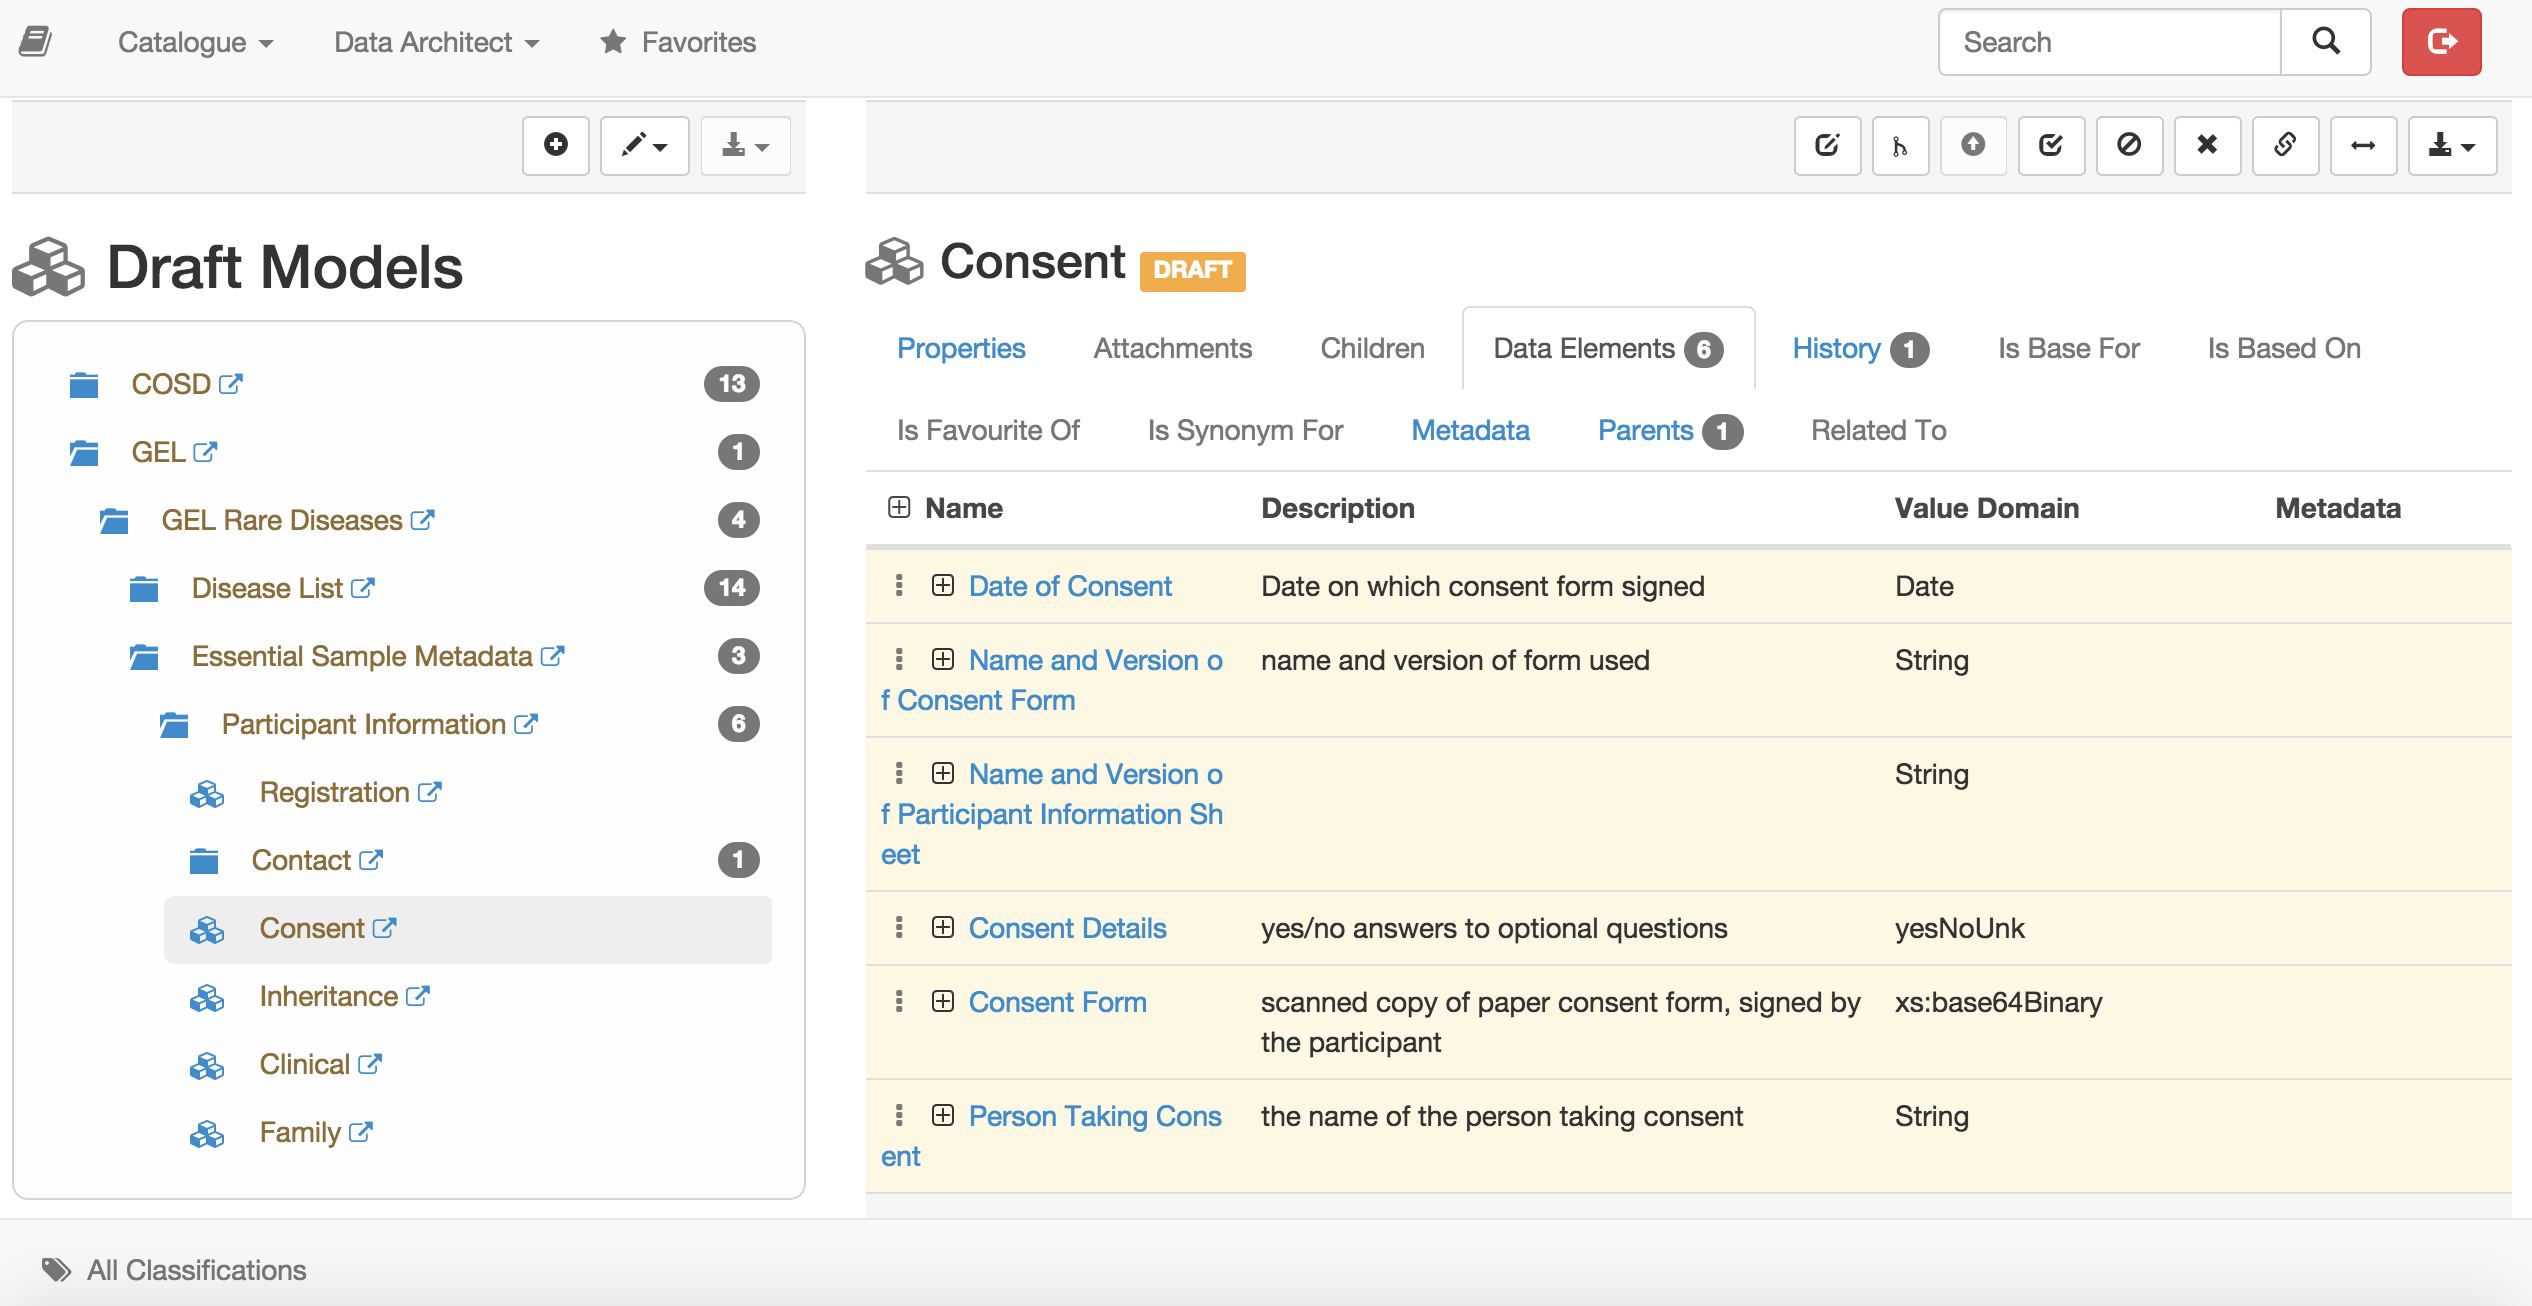
\includegraphics[width=\textwidth]{ScreenShot1}
  \caption{web interface to the model catalogue}
  \label{fig:webinterface}
\end{figure*}

\begin{figure*}[h]
  \centering
  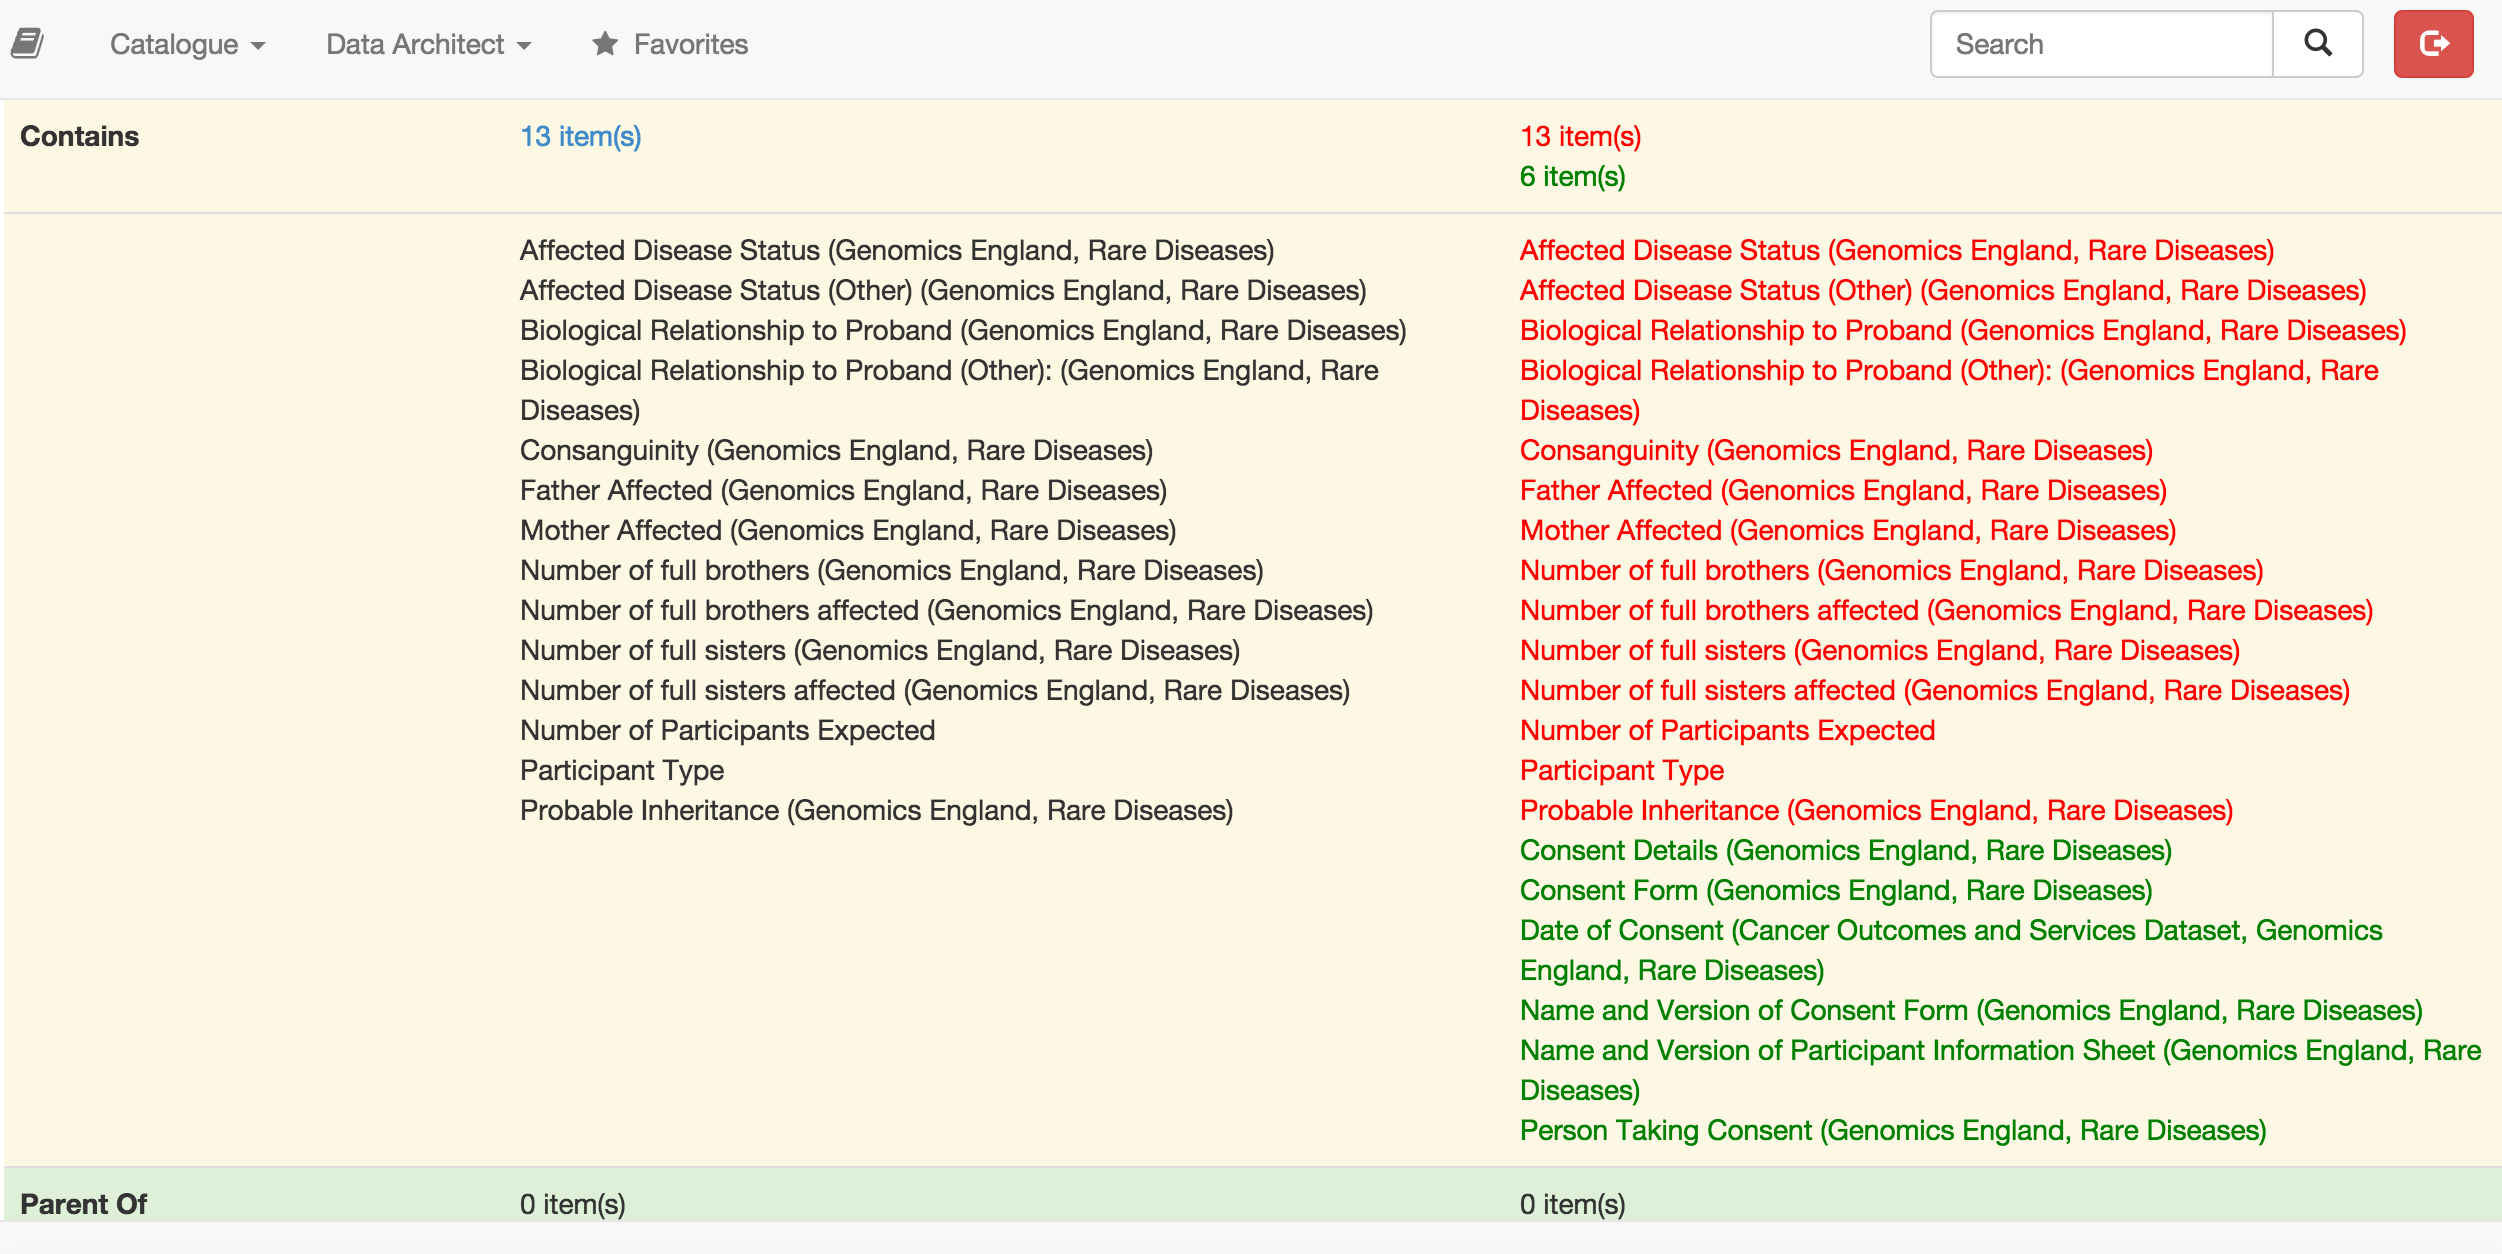
\includegraphics[width=\textwidth]{ScreenShot2}  
  \caption{automatic detection of model variation}
  \label{fig:variation}
\end{figure*}


 


\newpage

\bibliographystyle{IEEEtran}

\bibliography{ASEPub}


\end{document}  

%%% Local Variables:
%%% mode: latex
%%% TeX-master: "ASE2015MDR"
%%% End:
